\documentclass[a4paper, 10pt, dvipdfmx]{jlreq}

\usepackage{amsmath,amsfonts,amssymb}
\usepackage{bm}
\usepackage{mathtools}
\usepackage{siunitx}
\usepackage[dvipdfmx]{graphicx}
\usepackage[dvipdfmx]{color}
\usepackage[dvipdfmx, colorlinks=true, allcolors=blue]{hyperref}
\usepackage{listings, jlisting}
\usepackage{tikz}
\usepackage{physics}
\usepackage{url}

\Urlmuskip=0mu plus 10mu
\allowdisplaybreaks[4]
\frenchspacing
\definecolor{OliveGreen}{rgb}{0.0,0.6,0.0}
\definecolor{Orenge}{rgb}{0.89,0.55,0}
\definecolor{SkyBlue}{rgb}{0.28, 0.28, 0.95}
\lstset{
  language={c++},
  basicstyle={\ttfamily},
  identifierstyle={\small},
  ndkeywordstyle={\small},
  frame=single,
  breaklines=true,
  numbers=left,
  xrightmargin=0zw,
  xleftmargin=3zw,
  numberstyle={\scriptsize},
  lineskip=-0.9ex,
  keywordstyle={\small\bfseries\color{SkyBlue}},
  commentstyle={\color{OliveGreen}},
  stringstyle={\small\ttfamily\color{Orenge}}
}

\begin{document}

\title{k-RDMの高速化手法について}
\author{計数工学科 3 年 03-220602 浜口広樹}
\date{\today}
\maketitle

\section{問題設定}


kRDMを求めよ。必要な計算量はいくらほどか。

\section{行列積}

まず、先んじて以下の行列を考えます。

\begin{align*}
      & \text{jordan\_wigner\_ladder\_sparse}(Q,a,0)     \\
    = & \mqty(1                                      & 0 \\ 0 & -1)^a \otimes \mqty(0&1\\0&0) \otimes I_{2^{Q-a-1}} \\
\end{align*}

ただし、$\otimes$はクロネッカー積を表すとし、累乗に関してもクロネッカー積に関するものです。(書き方の流儀が分かりませんが…)(また、先日この関数の定義が分からないと私が騒いでいましたが、ちゃんと落ち着いて読めば分かりました。申し訳ありません。)

この時、その内$k$個を選んだ際の順列に関する積が必要なので、それを求めます。

\newpage

\begin{figure}[htbp]
    \begin{minipage}{0.45\hsize}
        \begin{center}
            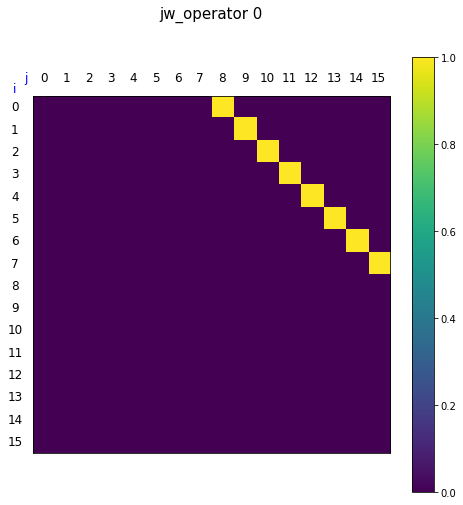
\includegraphics[width=60mm]{jw_operators/0.png}
        \end{center}
        \caption{0番目}
    \end{minipage}
    \begin{minipage}{0.45\hsize}
        \begin{center}
            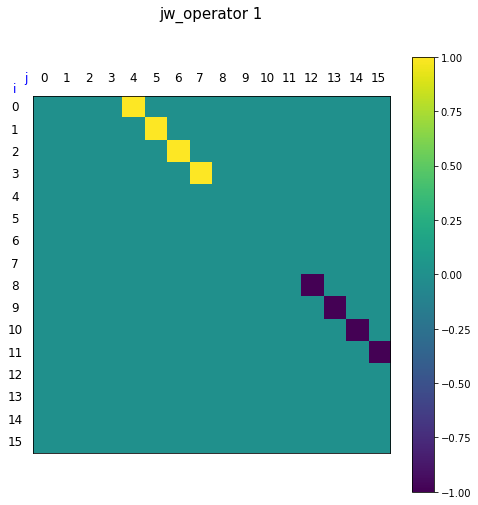
\includegraphics[width=60mm]{jw_operators/1.png}
        \end{center}
        \caption{1番目}
    \end{minipage}
\end{figure}
\begin{figure}[htbp]
    \begin{minipage}{0.45\hsize}
        \begin{center}
            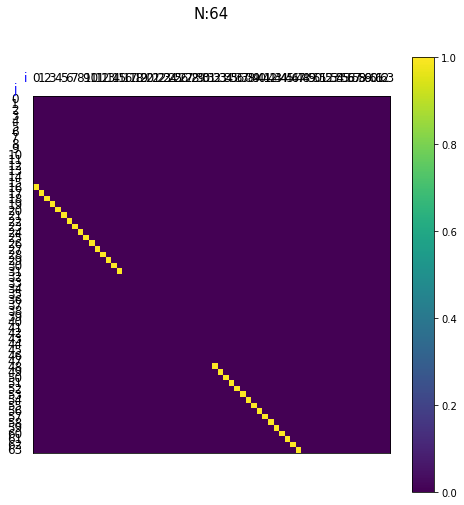
\includegraphics[width=60mm]{jw_operators/2.png}
        \end{center}
        \caption{2番目}
    \end{minipage}
    \begin{minipage}{0.45\hsize}
        \begin{center}
            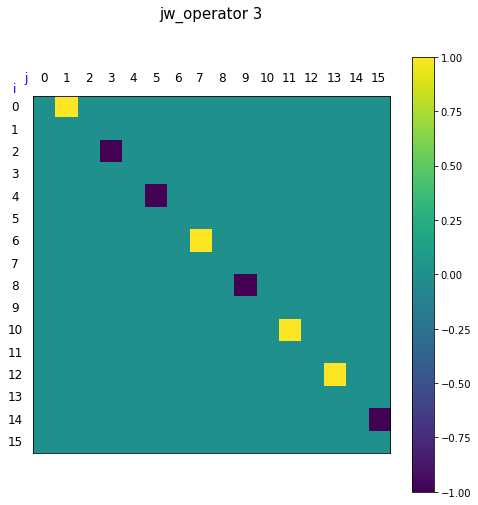
\includegraphics[width=60mm]{jw_operators/3.png}
        \end{center}
        \caption{3番目}
    \end{minipage}
\end{figure}

\newpage

\section{行列積の演算}

以下で求められます。

\begin{lstlisting}[caption=Python, label=code:answer, language=Python]
def _make_jordan_wigners_mul_vec(Q: int, k: int, vec: np.ndarray,
                                 ) -> Dict[int, np.ndarray]:
    assert 1 <= k <= Q

    n_hilbert = 2**Q
    jordan_wigners_mul_vec = dict()

    for ps in combinations(range(Q)[::-1], k):
        data = []
        row = []
        col = []
        offset = sum(1 << (Q-1-p) for p in ps)
        mask = (n_hilbert-1) ^ offset
        r = n_hilbert-offset
        while r > 0:
            r = (r-1) & mask
            data.append(+1 if (sum(bin(r >> (Q-1-p))[2:].count('1')
                                   for p in ps) % 2 == 0) else -1)
            row.append(r)
            col.append(r+offset)

        ans = csr_matrix((data, (row, col)),
                         shape=(n_hilbert, n_hilbert)) @ vec
        jordan_wigners_mul_vec[_getIdx(Q, *ps)] = ans
        jordan_wigners_mul_vec[_getIdx(Q, *ps[::-1])] =\
            ans*((-1)**((k*(k-1)//2) % 2))

    return jordan_wigners_mul_vec
\end{lstlisting}

その理由を、大筋だけですが以下に書きます。

関数$f(i,P) : \mathbb{N} \times \mathbb{N}^\mathbb{N} \to \pm 1$を以下の様に定義します。

\begin{align*}
    f(i,P)=
    \begin{cases}
        +1 & (\sum_{p \in P}{\text{popcount}\left(i>>p\right)}+\epsilon(P) \equiv 0 \mod{2}) \\
        -1 & (\text{otherwise})
    \end{cases}
\end{align*}

ただし、関数$\text{popcount}(i): \mathbb{N} \to \mathbb{N}$は、$i$を二進数表記した際の1の個数(立っているビット数)とし、
$i>>p$で$i$を$p$桁右シフトした値($\left\lfloor\frac{i}{2^p}\right\rfloor$)を表すものとします。

また、$\&$は2進数表記した際のbit毎のandを示すものとし、$\text{bitsum}(P)=\sum_{p \in P}{2^p}$とします。

すると、求めるべき行列の$i$行$j$列成分に対して、$P$を掛け合わせる行列の添字列として、

\begin{quote}
    \begin{itemize}
        \item 上から右への斜め線状に要素があること: $\delta_{i+\text{bitsum}(P),j}$
        \item 要素が零かどうかの規則: $i\&\text{bitsum}(P)=0$
        \item 要素の符号についての規則: $f(i,P)$
    \end{itemize}
\end{quote}

という条件で示されることが分かり、これが演算を通して常に成立する不変条件となることが、帰納法により確かめられます。

よって、正当性が示されます。

ちなみに、実装上の工夫として、所謂\href{https://qiita.com/drken/items/7c6ff2aa4d8fce1c9361#7-%E4%B8%8E%E3%81%88%E3%82%89%E3%82%8C%E3%81%9F%E9%83%A8%E5%88%86%E9%9B%86%E5%90%88%E3%81%AE%E9%83%A8%E5%88%86%E9%9B%86%E5%90%88%E3%82%92%E5%88%97%E6%8C%99}{3乗のdp}と呼ばれる問題に対するコードを一部活用しています。

\section{kRDM}

以上の議論を基に、kRDMを求めます。
コードを読む方が早い気もするので、以下に載せます。
方針はslackにて共有して頂いたものの、ほぼそのまま(なはず)です。

\begin{lstlisting}[caption=kRDM, label=code:kRDM, language=Python]
def fast_compute_k_rdm(k: int, vec: np.ndarray,
                       verbose: bool = True) -> np.ndarray:
    Q = int(np.log2(vec.shape[0]))
    assert 2**Q == vec.shape[0]

    # 要請: k <= Q でなければならない(そうでなければ全て0)
    assert 1 <= k <= Q

    QCk = factorial(Q)//factorial(k)//factorial(Q-k)
    QPk = factorial(Q)//factorial(Q-k)

    rdm_data = [0j]*(QPk**2)
    rdm_idx = [0]*(QPk**2)

    fixed_k = _generate_fixed_parity_permutations(k)

    jordan_wigners_mul_vec = _make_jordan_wigners_mul_vec(Q, k, vec)

    idx_up = Q**k

    i = 0
    for ps, qs in tqdm(combinations(combinations(range(Q), k), 2),
                       total=QCk*(QCk-1)//2,
                       disable=not verbose):
        bra = jordan_wigners_mul_vec[_getIdx(Q, *ps[::-1])]
        ket = jordan_wigners_mul_vec[_getIdx(Q, *qs)]
        val = np.dot(bra.conj(), ket)
        val_conj = val.conj()

        for perm1, parity1 in _generate_parity_permutations(ps, fixed_k):
            val_p1 = val*parity1
            val_conj_p1 = val_conj*parity1
            idx1 = _getIdx(Q, *perm1)
            for perm2, parity2 in _generate_parity_permutations(qs, fixed_k):
                idx2 = _getIdx(Q, *perm2)
                rdm_idx[i] = idx1*idx_up+idx2
                rdm_data[i] = val_p1*parity2
                i += 1
                rdm_idx[i] = idx2*idx_up+idx1
                rdm_data[i] = val_conj_p1*parity2
                i += 1

    for ps in combinations(range(Q), k):
        bra = jordan_wigners_mul_vec[_getIdx(Q, *ps[::-1])]
        ket = jordan_wigners_mul_vec[_getIdx(Q, *ps)]
        val = np.dot(bra.conj(), ket)
        val_conj = val.conj()
        gpp = _generate_parity_permutations(ps, fixed_k)
        for perm1, parity1 in gpp:
            val_p1 = val*parity1
            idx1 = _getIdx(Q, *perm1)
            for perm2, parity2 in gpp:
                idx2 = _getIdx(Q, *perm2)
                rdm_idx[i] = idx1*idx_up+idx2
                rdm_data[i] = val_p1*parity2
                i += 1

    return coo_matrix((rdm_data, ([0]*len(rdm_data), rdm_idx)),
                      shape=(1, Q**(2*k)), dtype=complex)\
        .toarray()\
        .reshape(tuple(Q for _ in range(2*k)))
\end{lstlisting}

\section{計算量}

非零要素数は$({}_Q P_k)^2$個あり、その内でwedge積同様の同値類(「up to signで等しい」もの)のような考え方をすると、本当に必要な要素は${}_{{}_Q C_k} C_2+{}_Q C_k$個です。

前者が上側と下側で添字集合が異なる場合、後者が上側と下側で添字集合が同一の場合を表します。

また、各同値類の代表元を求めるのに必要な計算量は、代表元を添字に関してソートされたものにすれば、転倒数(物理で言うと$\epsilon(P)$)を求めるのに必要な計算などをスキップできるので、前計算された$c_{j_1} ... c_{j_k} | \psi >$(ベクトル)同士の内積だけで計算出来て、これは$2^Q$だけで可能です。

そして、$c_{j_1} ... c_{j_k} | \psi >$の前計算は、先程の議論と、「代表元を添字に関してソートされたもの」にするという話から、$\order{2^Q}$で出来ます。(実際はもっと少ない)

以上より、

$$
    \order{2^Q {}_Q C_k + 2^Q({}_{{}_Q C_k} C_2+{}_Q C_k) + ({}_Q P_k)^2}
$$

が計算量となります。
第一項が前計算、第二項が代表元の計算、第三項が非零要素を全て求めるのに必要な計算量です。

これまでの計算では前計算に行列積を使うので$(2^Q)^2$が必要でしたが、それが消えたので、

$$
    \order{2^Q({}_{{}_Q C_k} C_2+{}_Q C_k) + ({}_Q P_k)^2}
$$

と書くことも出来き、${}_{{}_Q C_k} C_2 >> {}_Q C_k$なので、

$$
    \order{2^Q({}_{{}_Q C_k} C_2) + ({}_Q P_k)^2}
$$

と書くことも出来ます。

尤も、実測上は、そこはあまりボトルネックになっていなかったので、高々50秒中の2,3秒が縮んだ程度です。

\section{課題点}

この時、$Q=10,k=4$で、上の式は4.830e+07という数値を示すのですが、それと照らし合わせると計算の遅さが際立って個人的には非常に悔しいです。

本来、この計算量に対しては(1e7/secと考えると)4秒くらいで終わってもおかしくないはずなのですが、私の実装が悪いのか、あるいは素のPythonの限界なのか、40秒くらいは掛かります。

(wedge積に関しても同様で、演算回数がざっと1e6/secという結果になります。私は普段競プロでPythonを殆ど使わないので、肌感覚が少しおかしいのかも知れませんが、それにしてもやはり遅そうです)

これに関して、実はここ何日かなり定数倍改善の試行錯誤をしていたのですが、どうにも分からずお手上げ状態に近いです。Cythonも試そうとはしましたが、色々なモジュールにこのコードが依存している以上、流石に労力に対するリターンが少ないかなという気でいます。

尤も、wedge積も含めて、計算機のメモリに載る範囲内では殆どのケースがかなり高速に動作するはずです。

以上です。

\end{document}

